\section{Problem 5}
Transfer function to state space.

For each of the transfer functions shown, write the corresponding differential equation and provide a state space representation.
\subsection{a)}
\begin{equation}
    \frac{\Theta_1(s)}{T_1(s)} = \frac{100}{s^4+20s^3+10s^2+7s+100}
\end{equation}
\subsubsection{\textit{ Sol. }}
Convert the given transfer function to standard format:
$\frac{\Theta_1(s)}{T_1(s)} = \frac{b_1s^3+b_2s^2+b_3s+b_4}{s^4+a_1s^3+a_2s^2+a_3s+a_4}$, 

where $b_1 = b_2=b_3=0$, $b_4 = 100$, $a_1 = 20$, $a_2 = 10$, $a_3 = 7$, $a_4 = 100$.

We have:
\begin{equation}
    \begin{aligned}
        \dot{\textbf{x}} &=
        \begin{bmatrix}
            0    & 1    & 0    & 0\\
            0    & 0    & 1    & 0\\
            0    & 0    & 0    & 1\\
            -a_4 & -a_3 & -a_2 & -a_1
        \end{bmatrix}
        \textbf{x} + 
        \begin{bmatrix}
            0 \\ 0 \\ 0 \\ 1
        \end{bmatrix}
        u \\ &=
        \begin{bmatrix}
            0    & 1    & 0    & 0\\
            0    & 0    & 1    & 0\\
            0    & 0    & 0    & 1\\
            -100 & -7   & -10  & -20
        \end{bmatrix}
        \textbf{x} + 
        \begin{bmatrix}
            0 \\ 0 \\ 0 \\ 1
        \end{bmatrix}
        u \\
        y &=
        \begin{bmatrix}
            b_4 & b_3 & b_2 & b_1
        \end{bmatrix}
        \textbf{x} + 
        \begin{bmatrix}
            0
        \end{bmatrix}
        u \\ &=
        \begin{bmatrix}
            100 & 0 & 0 & 0
        \end{bmatrix}
        \textbf{x} + 
        \begin{bmatrix}
            0
        \end{bmatrix}
        u
    \end{aligned}
\end{equation}

Matlab code:
    \lstinputlisting{codes/Question5a.m}
Result:
\begin{figure}[htp]
    \centering
    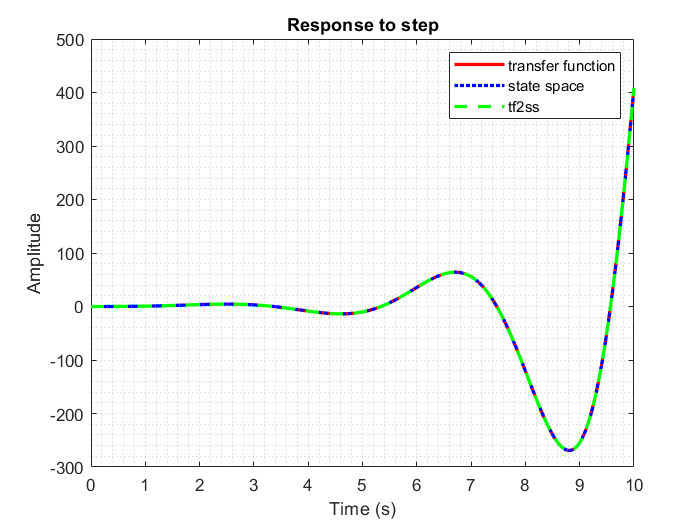
\includegraphics[width=12cm]{images/Q5_a_fig.png}
    \caption{Step Response}
    \label{fig:Q5a1}
\end{figure}


\subsection{b)}
\begin{equation}
    \frac{Y_1(s)}{F_1(s)} = \frac{8s+10}{s^3+s^2+5s+13}
\end{equation}

\subsubsection{\textit{ Sol. }}
Convert the given transfer function to standard format:
$\frac{Y_1(s)}{F_1(s)} = \frac{b_1s^2+b_2s+b_3}{s^3+a_1s^2+a_2s+a_3}$, 

where $b_1 =0$, $b_2=8$, $b_3 = 10$, $a_1 = 1$, $a_2 = 5$, $a_3 = 13$.

We have:
\begin{equation}
    \begin{aligned}
        \dot{\textbf{x}} &=
        \begin{bmatrix}
            0    & 1    & 0\\
            0    & 0    & 1\\
            -a_3 & -a_2 & -a_1
        \end{bmatrix}
        \textbf{x} + 
        \begin{bmatrix}
            0 \\ 0 \\ 1
        \end{bmatrix}
        u \\ &=
        \begin{bmatrix}
            0    & 1    & 0\\
            0    & 0    & 1\\
            -13  & -5   & -1
        \end{bmatrix}
        \textbf{x} + 
        \begin{bmatrix}
            0 \\ 0 \\ 1
        \end{bmatrix}
        u \\
        y &=
        \begin{bmatrix}
            b_3 & b_2 & b_1
        \end{bmatrix}
        \textbf{x} + 
        \begin{bmatrix}
            0
        \end{bmatrix}
        u \\ &=
        \begin{bmatrix}
            10 & 8 & 0
        \end{bmatrix}
        \textbf{x} + 
        \begin{bmatrix}
            0
        \end{bmatrix}
        u
    \end{aligned}
\end{equation}

Matlab code:
    \lstinputlisting{codes/Question5b.m}
Result:
\begin{figure}[htp]
    \centering
    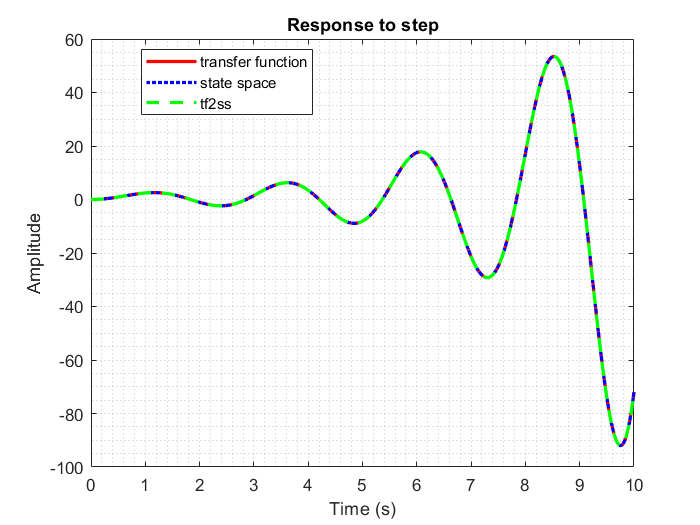
\includegraphics[width=12cm]{images/Q5_b_fig.png}
    \caption{Step Response}
    \label{fig:Q5a1}
\end{figure}
\pagebreak